\documentclass[border=10pt]{standalone}

\usepackage{tikz}
\usepackage{tikzsymbols}
\usetikzlibrary{calc,patterns,shapes.geometric}

\def\centerarc[#1](#2)(#3:#4:#5){\draw[#1] ($(#2)+({#5*cos(#3)},{#5*sin(#3)})$) arc (#3:#4:#5);}

\begin{document}
	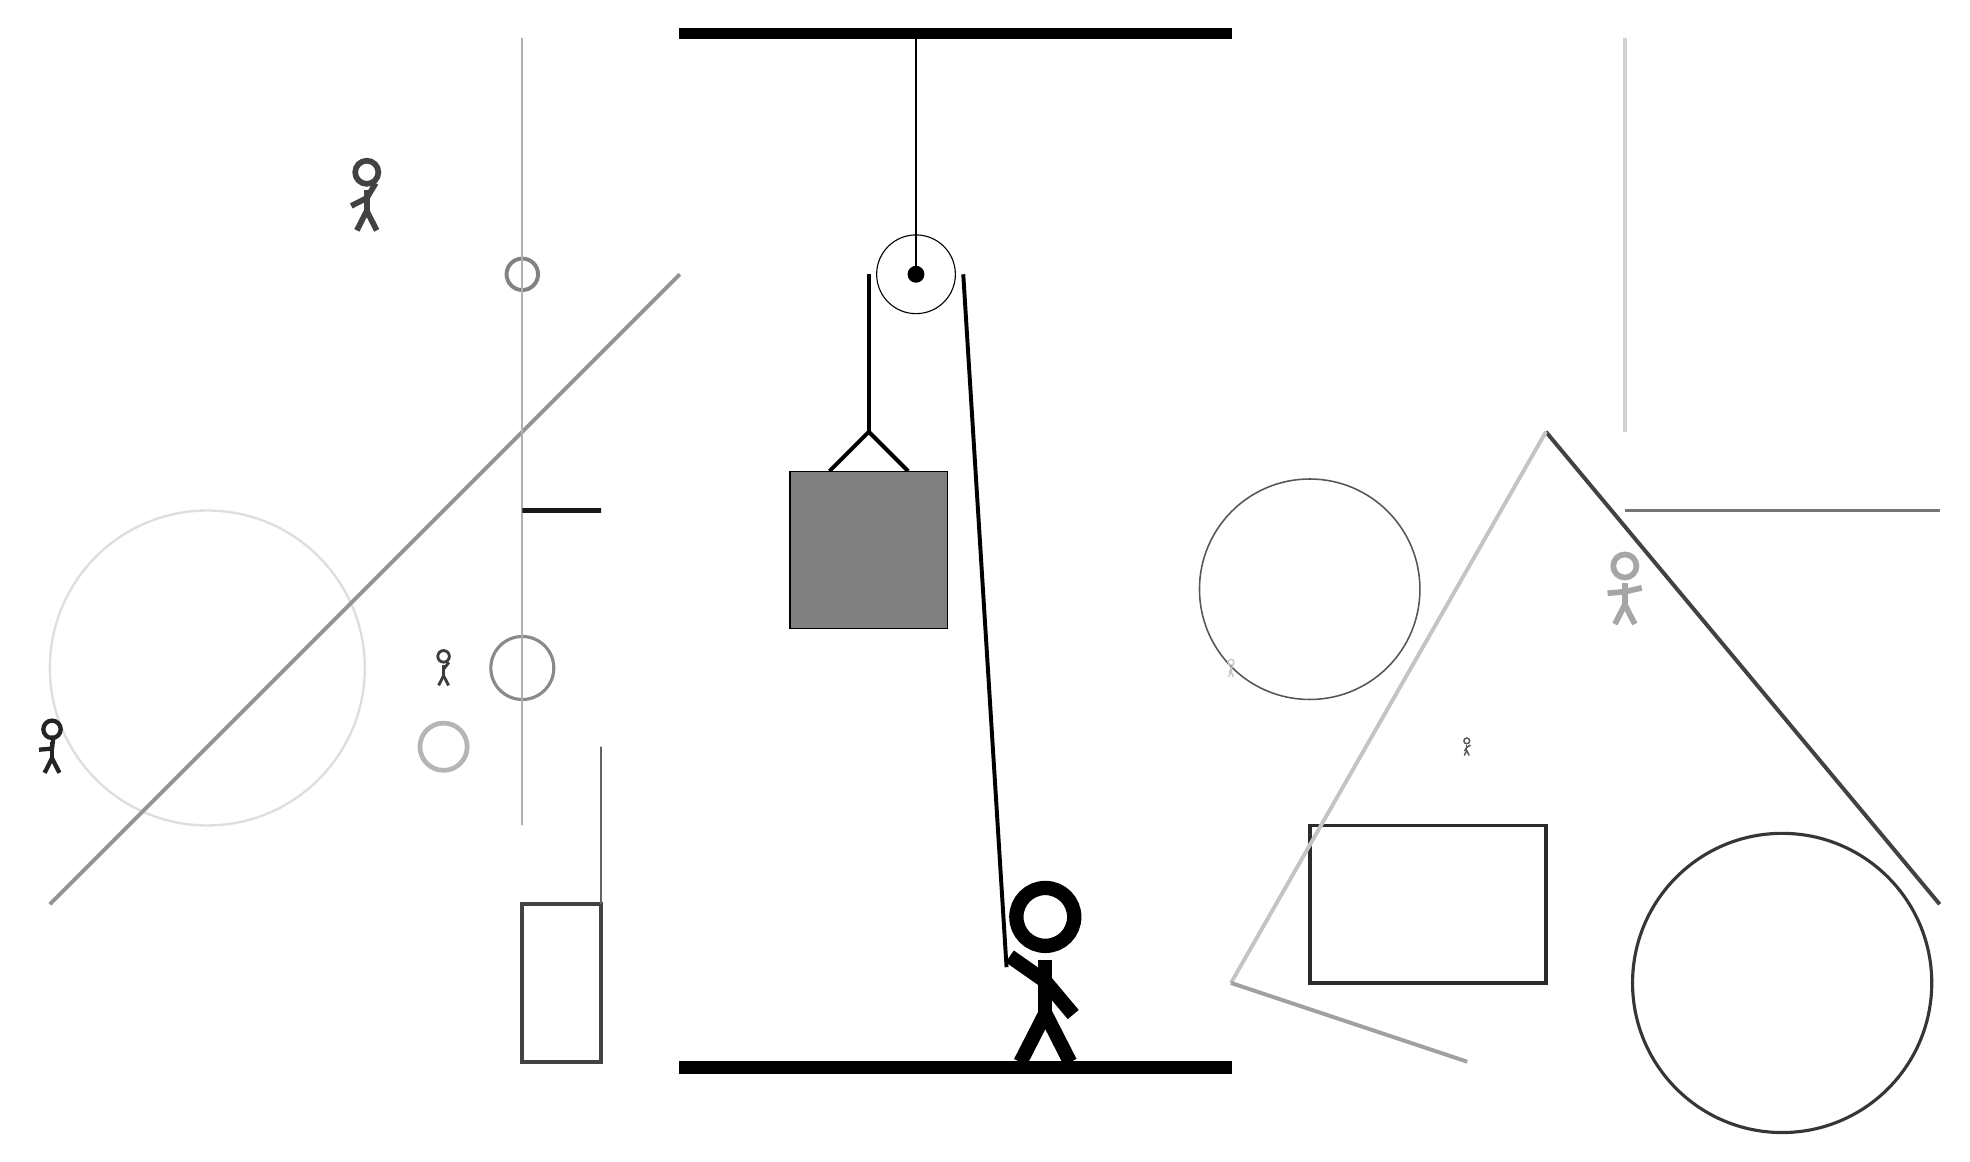
\begin{tikzpicture}
		%%%%% START %%%%%
		
		\draw[fill=black] (-2, 10) rectangle (5, 10.125);
		
		\draw [line width=0.4mm, color=black!79](12, -2) circle (1.9);
		
		\draw[line width=0.5mm, color=black!83] (6, 0) rectangle (9, -2);
		\draw [line width=0.5mm, color=black!49](-4, 7) circle (0.2);
		\draw [line width=0.2mm, color=black!66](6, 3) circle (1.4);
		\draw[line width=0.5mm, color=black!74](9, 5) -- (14, -1);
		\draw[line width=0.5mm, color=black!23](9, 5) -- (5, -2);
		\node[line width=0.3mm, color=black!68] at (8, 1) {\Strichmaxerl[1][58][31]};
		\node[line width=0.6mm, color=black!22] at (5, 2) {\Strichmaxerl[1][67][54]};
		\draw [line width=0.3mm, color=black!13](-8, 2) circle (2.0);
		
		\draw[line width=0.5mm, color=black!42](-2, 7) -- (-10, -1);
		\draw [line width=0.4mm, color=black!46](-4, 2) circle (0.4);
		
		\node[line width=0.7mm, color=black!35] at (10, 3) {\Strichmaxerl[4][5][13]};
		\draw[line width=0.5mm, color=black!74] (-4, -1) rectangle (-3, -3);
		\node[line width=0.6mm, color=black!74] at (-6, 8) {\Strichmaxerl[4][27][59]};
		\draw[line width=0.5mm, color=black!18](10, 5) -- (10, 10);
		\node[line width=0.3mm, color=black!76] at (-5, 2) {\Strichmaxerl[2][90][52]};
		\draw[line width=0.3mm, color=black!31] (-4, 10) rectangle (-4, 0);
		
		\draw[line width=0.2mm, color=black!61] (-3, 1) rectangle (-3, -1);
		\draw[line width=0.7mm, color=black!91] (-4, 4) rectangle (-3, 4);
		
		\draw[line width=0.5mm, color=black!54](10, 4) -- (14, 4);
		\draw[line width=0.5mm, color=black!37](8, -3) -- (5, -2);
		\node[line width=0.5mm, color=black!86] at (-10, 1) {\Strichmaxerl[3][5][83]};
		\draw [line width=0.7mm, color=black!21](7, 7) circle (0.0);
		\draw [line width=0.6mm, color=black!29](-5, 1) circle (0.3);
		
		\draw (1, 7) circle (0.5);
		\draw[fill=black] (1, 7) circle (0.1);
		\draw (1, 10) -- (1, 7);
		
		\draw[line width=0.5mm] (-0.1, 4.5) -- (0.4, 5.0) -- (0.9, 4.5);
		\draw[fill=black!50] (-0.6, 4.5) rectangle (1.4, 2.5);
		
		\draw[line width=0.5mm] (0.4, 7) -- (0.4, 5.0);
		\centerarc[line width=0.5mm](1, 7)(0:180:0.6);
		\draw[line width=0.5mm](1.6, 7) -- (2.15, -1.8);
		
		\node at (2.6, -1.9) {\Strichmaxerl[10][-35][-50]};
		
		\draw[fill=black] (-2, -3) rectangle (5, -3.15);
		
		%%%%% END %%%%%
	\end{tikzpicture}
\end{document}